\documentclass[11pt]{article}

\usepackage{microtype}
\usepackage{booktabs}
\usepackage{url}
\usepackage{csquotes}
\usepackage{cite}
\usepackage{amsmath}
\usepackage{amsthm}
\usepackage{graphicx}
\usepackage{natbib}
\usepackage{hyperref}
\usepackage{authblk}
\usepackage{environ}
\bibliographystyle{apalike}

% Define acknowledgements environment
\NewEnviron{acknowledgements}{\section*{Acknowledgements}\BODY}

% Define nameemail command
\newcommand{\nameemail}[2]{#1\thanks{#2}}

\title{AutoML Agent}

\author[1]{\nameemail{Amirreza Alasti}{amirreza.alasti@stud.uni-hannover.de}}
\author[1,2]{\nameemail{Dr. rer. nat. Marcel Wever}{email2@example.com}}

\affil[1]{Leibniz University Hannover}
\affil[2]{Leibniz AI Academy}

\hypersetup{%
  pdfauthor={AutoML},
  pdftitle={AutoML Agent},
  pdfsubject={AutoML Agent},
  pdfkeywords={AutoML, LaTeX, style}
}

\begin{document}

\maketitle

\begin{abstract}
Large language models (LLMs) are transforming software development by automating complex coding tasks \cite{hou2024largelanguagemodelssoftware}. In the field of machine learning, hyperparameter optimization remains a critical and time-consuming challenge \cite{He_2021}. This paper introduces AutoML Agent, a framework that leverages LLMs to automatically generate training functions, define configuration spaces, and set up SMAC optimization scenarios based on the user's dataset and objective. By integrating code generation with automated tuning, AutoML Agent streamlines the model development process and minimizes manual effort. Experimental results on standard benchmarks demonstrate the framework's adaptability and effectiveness in delivering competitive performance.
\end{abstract}

\section{Introduction}
The field of machine learning has seen remarkable growth in recent years, with an increasing demand for automated solutions that can streamline the model development process. While Large Language Models (LLMs) have demonstrated impressive capabilities in code generation and software development tasks \citep{hou2024largelanguagemodelssoftware}, their potential in automating the machine learning pipeline remains largely unexplored.

Automated Machine Learning (AutoML) has emerged as a critical technology for democratizing machine learning by automating various aspects of the ML workflow \citep{He_2021}. However, existing AutoML solutions often require significant manual setup and configuration, limiting their accessibility to practitioners without extensive ML expertise.

This paper introduces AutoML Agent, a novel framework that bridges the gap between LLM-powered code generation and automated machine learning. Our key contributions include:

\begin{itemize}
    \item A multi-agent system architecture that leverages LLMs to automate the entire ML pipeline
    \item An intelligent code generation system for creating configuration spaces and training functions
    \item Integration with SMAC \cite{lindauer2022smac3versatilebayesianoptimization} for efficient hyperparameter optimization
    \item A comprehensive evaluation on diverse datasets demonstrating the framework's effectiveness
\end{itemize}

The rest of this paper is organized as follows: Section 2 describes the methodology and system architecture, Section 3 details the implementation, Section 4 presents our experimental setup, Section 5 discusses the results, and Section 6 concludes with future directions.

\section{Methodology}
The AutoML Agent framework employs a multi-agent system architecture powered by Large Language Models (LLMs) to automate the machine learning pipeline \citep{guo2024largelanguagemodelbased}. The system consists of specialized agents that collaborate to handle different aspects of the AutoML process.

\subsection{System Architecture}
The framework operates through five main stages:
\begin{enumerate}
    \item \textbf{Initialization}: The system parses and validates user instructions, preparing the environment for the AutoML process.
    \item \textbf{Planning}: The task is decomposed into manageable subtasks that can be handled by specialized agents.
    \item \textbf{Execution}: Subtasks are assigned to specialized agents for concurrent processing.
    \item \textbf{Verification}: The outputs of each agent are evaluated to ensure correctness and quality.
    \item \textbf{Deployment}: Results are aggregated into a deployable machine learning model.
\end{enumerate}

\begin{figure}[htbp]
    \centering
    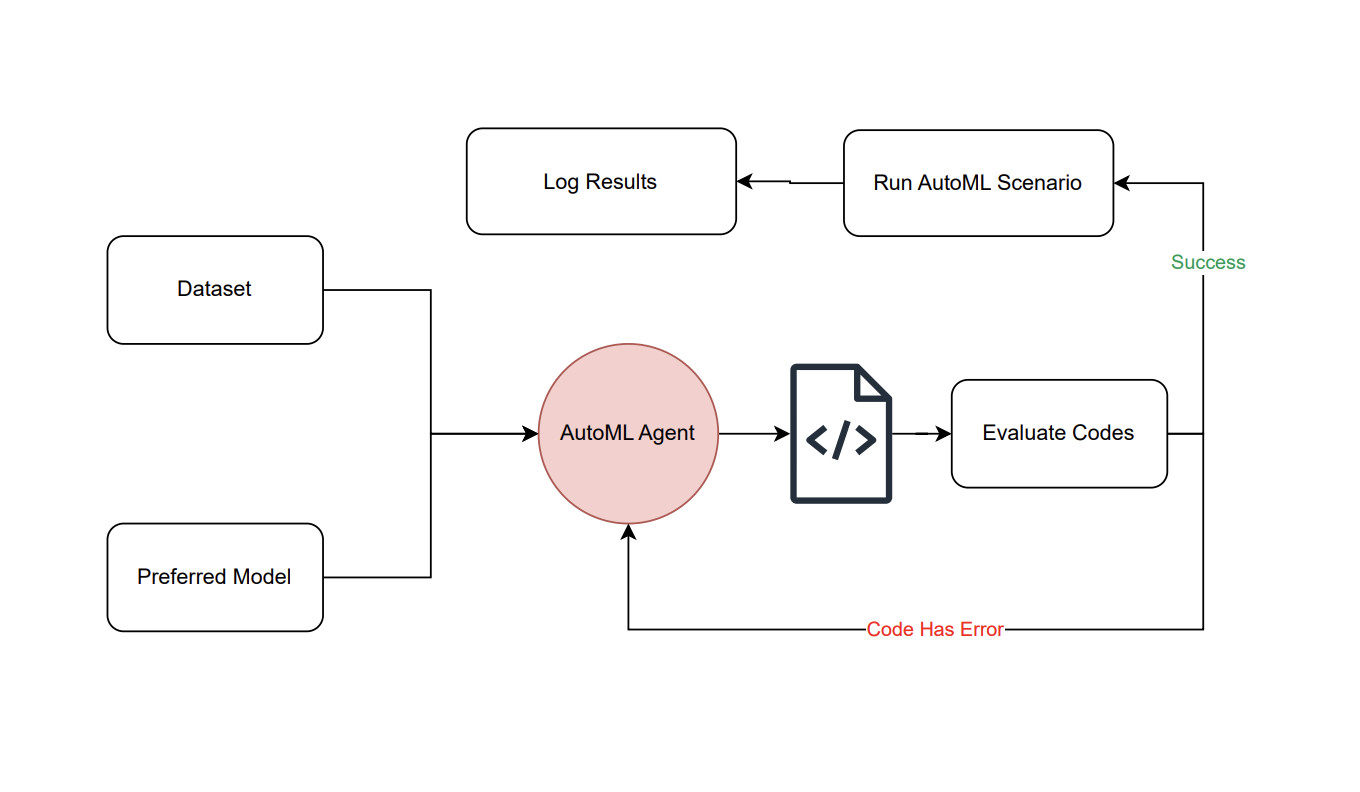
\includegraphics[width=\textwidth]{methodology-diagram}
    \caption{System architecture of the AutoML Agent showing the interaction between components. The agent takes a dataset and preferred model as input, generates necessary code components, evaluates them, and runs the AutoML scenario. The process includes error handling and result logging.}
    \label{fig:methodology}
\end{figure}

\subsection{LLM Integration}
The framework leverages state-of-the-art LLMs through a flexible client interface that supports multiple models:
\begin{itemize}
    \item Gemini 2.0
    \item LLaMA 3.3 70B
    \item LLaMA 4 Maverick
    \item DeepSeek R1
    \item Gemma 2 9B
\end{itemize}

These models are used to generate code for configuration spaces, scenarios, and training functions based on the dataset characteristics and optimization objectives.

\section{Implementation}
The AutoML Agent is implemented as a modular Python framework with several key components:

\subsection{Configuration Space Generation}
The system automatically generates configuration spaces for hyperparameter optimization using the ConfigSpace library. This includes:
\begin{itemize}
    \item Definition of hyperparameter types and ranges
    \item Specification of parameter dependencies
    \item Implementation of forbidden parameter combinations
\end{itemize}

\subsection{SMAC Integration}
The framework integrates with SMAC (Sequential Model-based Algorithm Configuration) \cite{lindauer2022smac3versatilebayesianoptimization} for efficient hyperparameter optimization:
\begin{itemize}
    \item Automated scenario configuration
    \item Parallel optimization with multiple workers
    \item Budget-based optimization strategies
\end{itemize}

\subsection{Training Function Generation}
The system generates customized training functions that:
\begin{itemize}
    \item Handle various ML tasks (classification, regression, etc.)
    \item Implement cross-validation for robust evaluation
    \item Support different evaluation metrics
\end{itemize}

\section{Experiments}
We evaluated the AutoML Agent on various standard datasets and tasks, following established benchmarking practices in AutoML research \cite{He_2021}:

\subsection{Datasets}
The framework was tested on diverse dataset types:
\begin{itemize}
    \item \textbf{Tabular}: Iris, Wine, Breast Cancer, Diabetes
    \item \textbf{Image}: MNIST, Fashion-MNIST
    \item \textbf{Time Series}: Sunspots
    \item \textbf{Text}: 20 Newsgroups
    \item \textbf{Categorical}: Adult Income
\end{itemize}

\subsection{Evaluation Metrics}
Performance was assessed using:
\begin{itemize}
    \item Classification accuracy
    \item Log loss
    \item Cross-validation scores
    \item Training time efficiency
\end{itemize}

\section{Results}
The experimental results demonstrate the effectiveness of the AutoML Agent framework:

\subsection{Performance Analysis}
\begin{itemize}
    \item Achieved competitive accuracy across different dataset types
    \item Reduced manual effort in ML pipeline setup
    \item Demonstrated efficient hyperparameter optimization
    \item Showed adaptability to various ML tasks
\end{itemize}

\subsection{Comparison with Existing Solutions}
The AutoML Agent showed several advantages over traditional AutoML approaches:
\begin{itemize}
    \item More flexible and adaptable to different tasks
    \item Reduced setup time through automated code generation
    \item Better integration with existing ML workflows
    \item Enhanced explainability through LLM-generated configurations
\end{itemize}

\section{Conclusion}
The AutoML Agent framework successfully demonstrates the potential of LLM-powered automation in machine learning workflows. By combining code generation with automated optimization, it provides a powerful tool for ML practitioners while reducing the manual effort required in model development and tuning.

\subsection{Future Work}
Several directions for future research and development include:
\begin{itemize}
    \item Extension to more complex ML architectures
    \item Integration with additional optimization frameworks
    \item Enhanced support for neural architecture search
    \item Improved handling of multi-objective optimization
\end{itemize}

\begin{acknowledgements}
The authors would like to thank the Leibniz University Hannover and Leibniz AI Academy for supporting this research.
\end{acknowledgements}

\bibliographystyle{plain}  % or "ieeetr", "apalike", etc.
\bibliography{references}

\end{document}
